\section{Index-Consistent Harmonic Projection}
\label{sec:method}

\subsection{Overview}

Given an univariate telemetry series, the frozen ViT4TS screen renders
overlapping windows as line images, extracts multiscale visual tokens with a
CLIP Vision Transformer (ViT), and compares the tokens with a median visual
memory built from all windows of that series~\cite{he2026vlm4ts,radford2021clip,dosovitskiy2021vit}. The resulting
token costs must then be returned to a common spatial grid before they can be
localized in time. Index-Consistent Harmonic Projection (IHP) changes only
this return map. As shown in Fig.~\ref{fig:ihp}, IHP restores the literal
token-to-cell support relation and evaluates the inherited harmonic projector
unchanged on that corrected support before the fixed scale fusion and
timestamp stitcher.

\begin{figure*}[t]
  \centering
  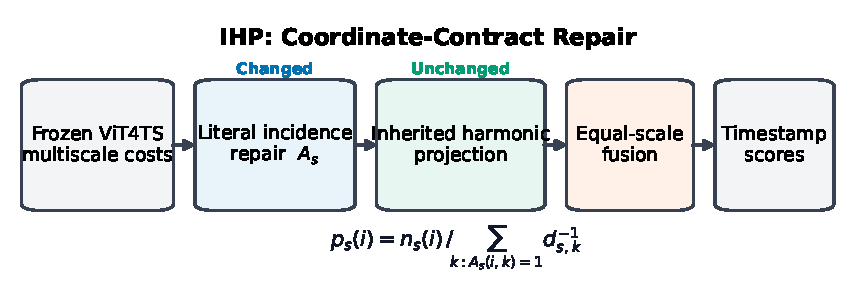
\includegraphics[width=0.98\textwidth]{figures/ihp_method.pdf}
  \caption{IHP is a coordinate-contract repair inside the frozen ViT4TS
  screen. Literal incidence repairs the released zero-based support relation;
  the inherited ViT4TS harmonic projector then aggregates the same frozen
  token costs unchanged on that corrected support. The encoder, visual memory,
  matching, scale fusion, and timestamp stitching remain fixed.}
  \label{fig:ihp}
\end{figure*}

The design follows a single causal chain. Section~\ref{sec:coordinate_failure}
defines the coordinate-contract failure. Sections~\ref{sec:literal_lifting}
and~\ref{sec:harmonic_pullback} present the repair and its inherited reducer, and
Section~\ref{sec:system_integration} specifies the frozen-system boundary and
computational properties. IHP has no training objective, learned parameter,
or label-dependent branch.

\subsection{Frozen Screening Interface}

Let a rendered window be encoded on a $g\times g$ base grid, where the frozen
ViT-B/16 configuration gives $g=14$ and $N=g^2=196$ base cells. We index a
base cell by $i\in\Omega=\{0,\ldots,N-1\}$ and use
$s\in\mathcal{S}=\{\mathrm{b},\mathrm{m},\mathrm{l}\}$ for the base, medium,
and large token scales. Their token counts are $K_{\mathrm{b}}=196$,
$K_{\mathrm{m}}=169$, and $K_{\mathrm{l}}=144$, corresponding to the base
grid and the released overlapping $2\times2$ and $3\times3$ pooling layouts.

For window $w$, let $d_{w,s,k}\geq0$ denote the frozen cosine-dissimilarity
cost of token $k$ at scale $s$. IHP does not alter how this cost is obtained:
the line renderer, CLIP weights, multiscale pooling, median memory, and
unrestricted nearest-memory comparison are fixed. For each pooled token, the
released assets also provide a set
$M_{s,k}\subseteq\Omega$ containing the flattened base-cell indices that
contributed to that token. These sets are the sole geometric input to IHP.

\subsection{Failure Mechanism: A Shifted Support Graph}
\label{sec:coordinate_failure}

We call a multiscale projector \emph{index-consistent} when the support used
to score output cell $i$ is exactly the set of tokens whose provided
membership contains $i$. However, the released implementation queries the
already zero-based memberships with a one-step shift. Its effective incidence
matrix is
\begin{equation}
 A^{\mathrm{rel}}_s(i,k)
 =\mathbb{1}\!\left[i+1\in M_{s,k}\right],
 \qquad i\in\Omega ,
 \label{eq:released_incidence}
\end{equation}
where $A^{\mathrm{rel}}_s(i,k)$ indicates whether scale-$s$ token $k$ is used
for output cell $i$, $M_{s,k}$ is the released zero-based membership set, and
$\mathbb{1}[\cdot]$ is the indicator function.

Equation~\eqref{eq:released_incidence} advances every support query by one
flattened cell. At each pooled scale, 195 of 196 queries return valid support,
but all 195 are displaced. Thirteen shifts, at indices
$13,27,\ldots,181$, wrap across a row boundary; the remaining valid queries
move within a row. The terminal output cell $i=195$ queries index 196, which
cannot occur in $M_{s,k}\subseteq\{0,\ldots,195\}$ and therefore has no
pooled-token support. A subsequent finite-value fallback converts this
structural hole into a zero anomaly contribution. The mismatch is thus a
localization failure at the frozen token-to-grid interface rather than a
shortage of encoder capacity.

\subsection{Literal Incidence Repair}
\label{sec:literal_lifting}

IHP first lifts each provided membership set into a literal incidence matrix:
\begin{equation}
 A_s(i,k)=\mathbb{1}\!\left[i\in M_{s,k}\right],
 \qquad A_s\in\{0,1\}^{N\times K_s}.
 \label{eq:literal_incidence}
\end{equation}
Here, $A_s(i,k)$ links base cell $i$ to pooled token $k$, $N=196$ is the
number of output cells, and $K_s$ is the number of tokens at scale $s$. The
base scale uses the identity incidence $A_{\mathrm{b}}=I_N$ because each base
token already corresponds to one output cell.

Literal lifting is needed because a flattened index has meaning only under
the coordinate convention that generated it. Equation~\eqref{eq:literal_incidence}
uses the stored convention directly and introduces neither a learned mapping
nor a corrective offset. Consequently, it preserves every supplied
token--cell relation while removing the one-cell displacement, including its
13 row wraps, in Eq.~\eqref{eq:released_incidence}.

\noindent\textbf{Complete-coverage property.}
Let $n_s(i)=\sum_{k=1}^{K_s}A_s(i,k)$ be the number of scale-$s$ tokens
incident to cell $i$. If the released pooling layout covers the base grid,
$\bigcup_{k=1}^{K_s}M_{s,k}=\Omega$, then
$n_s(i)\geq1$ for every $i\in\Omega$. This follows directly because each
covered index appears in at least one membership set. The supplied medium and
large masks satisfy this premise, so literal lifting produces valid support
for all 196 cells without interpolation or an artificial terminal value.

\subsection{Inherited Harmonic Projection on Corrected Support}
\label{sec:harmonic_pullback}

After support is restored, IHP pulls each pooled token cost back to every base
cell that contributed to it. For a pooled scale
$s\in\{\mathrm{m},\mathrm{l}\}$, let
$\mathcal{I}_s(i)=\{k:A_s(i,k)=1\}$ denote the incident token set. The
projected cost is
\begin{equation}
 p_{w,s}(i)=
 \begin{cases}
 0, & \min_{k\in\mathcal{I}_s(i)}d_{w,s,k}=0,\\[2pt]
 \displaystyle
 \frac{n_s(i)}{\sum_{k\in\mathcal{I}_s(i)}d_{w,s,k}^{-1}},
 & \text{otherwise}.
 \end{cases}
 \label{eq:harmonic_pullback}
\end{equation}
In Eq.~\eqref{eq:harmonic_pullback}, $p_{w,s}(i)$ is the scale-$s$ cost at
base cell $i$ for window $w$, $d_{w,s,k}$ is the frozen nonnegative token
cost, $\mathcal{I}_s(i)$ is the literal incident set, and $n_s(i)$ normalizes
for the number of incident tokens. The first branch is the exact zero convention used
by the implementation: an incident zero dissimilarity makes the harmonic
cost zero, so no numerical $\epsilon$ or tunable floor is introduced.

The harmonic reducer and its support normalization are inherited from
ViT4TS; IHP does not claim a new mean in isolation. Its evaluated output is
different from the released path because the unchanged reducer is composed
with the index-consistent support graph and is defined for every output cell.
The normalization prevents cells covered by more overlapping pooled tokens
from receiving a larger value merely because their support cardinality is
larger.

The three frozen scales are fused with the released equal-scale average,
\begin{equation}
 P_w(i)=\frac{1}{3}\left(
 d_{w,\mathrm{b},i}+p_{w,\mathrm{m}}(i)+p_{w,\mathrm{l}}(i)
 \right),
 \label{eq:scale_fusion}
\end{equation}
where $P_w(i)$ is the final base-grid cost for window $w$,
$d_{w,\mathrm{b},i}$ is the base-token cost at cell $i$, and the remaining
terms are the medium- and large-scale pullbacks from
Eq.~\eqref{eq:harmonic_pullback}. Thus, no scale weight is learned or selected
per dataset.

\subsection{Frozen-System Integration and Properties}
\label{sec:system_integration}

The vector $P_w\in\mathbb{R}^{196}$ is reshaped to $14\times14$, bilinearly
upsampled to $224\times224$, reduced with the released top-quarter column
mean, and stitched across overlapping windows using the released temporal
alignment. These operations, the anomaly threshold sweep, and the optional
downstream VLM verification are outside IHP and remain unchanged. The present
system evaluates the frozen visual screening stage; it does not attribute
language-model reasoning to IHP.

IHP is deterministic, training-free, and parameter-free. Constructing the
fixed incidence matrices and applying Eq.~\eqref{eq:harmonic_pullback} has the
same asymptotic projection complexity as the released membership queries.
Most importantly, IHP reuses the same rendered windows, frozen visual tokens,
memory, and token costs, so it adds no encoder forward pass. Test labels are
read only by the evaluator after complete score files have been committed;
they do not enter incidence construction, projection, fusion, or stitching.
